% \documentclass[aspectratio=169,notes]{beamer}
\documentclass[aspectratio=169]{beamer}
\usetheme[faculty=phil]{fibeamer}
\usepackage{polyglossia}
\setmainlanguage{english} %% main locale instead of `english`, you
%% can typeset the presentation in either Czech or Slovak,
%% respectively.
\setotherlanguages{russian} %% The additional keys allow
%%
%%   \begin{otherlanguage}{czech}   ... \end{otherlanguage}
%%   \begin{otherlanguage}{slovak}  ... \end{otherlanguage}
%%
%% These macros specify information about the presentation
\title[Theoretical Mechanics]{Theoretical Mechanics, Lab 3: KIN PLANE2} %% that will be typeset on the
\subtitle{Plane motion
\\ \ \\ \ 
         } %% title page.
\author{Oleg Bulichev}
%% These additional packages are used within the document:
\usepackage{ragged2e}  % `\justifying` text
\usepackage{booktabs}  % Tables
\usepackage{tabularx}
\usepackage{tikz}      % Diagrams
\usetikzlibrary{calc, shapes, backgrounds}
\usepackage{amsmath, amssymb}
\usepackage{url}       % `\url`s
\usepackage{listings}  % Code listings
% \usepackage{subfigure}
\usepackage{floatrow}
\usepackage{subcaption}
\usepackage{mathtools}
\usepackage{todonotes}
\usepackage{fontspec}
\usepackage{multicol}
\usepackage{pdfpages}
\usepackage{wrapfig}
\usepackage{animate}
\usepackage{booktabs}
\usepackage{multirow}
% \usepackage{graphicx}
\usepackage{colortbl}

\graphicspath{{resources/}}
\frenchspacing

\setbeamertemplate{caption}[numbered]
\usetikzlibrary{graphs}

% \usepackage[backend=biber,style=ieee,autocite=footnote]{biblatex}
% \addbibresource{biblio.bib}
% \DefineBibliographyStrings{english}{%
%   bibliography = {References},}

\newcommand{\oleg}[2][] {\todo[color=red, #1] {OLEG:\\ #2}}
\newcommand{\fbckg}[1]{\usebackgroundtemplate{\includegraphics[width=\paperwidth]{#1}}}%frame background

\usepackage[framemethod=TikZ]{mdframed}
\newcommand{\dbox}[1]{
\begin{mdframed}[roundcorner=3pt, backgroundcolor=yellow, linewidth=0]
\vspace{1mm}
{#1}
\vspace{1mm}
\end{mdframed}
}

\begin{document}
\setlength{\abovedisplayskip}{0pt}
\setlength{\belowdisplayskip}{0pt}
\setlength{\abovedisplayshortskip}{0pt}
\setlength{\belowdisplayshortskip}{0pt}

\fbckg{fibeamer/figs/title_page.png}
\frame[c]{\setcounter{framenumber}{0}
    \usebeamerfont{title}%
    \usebeamercolor[fg]{title}%
    \begin{minipage}[b][6.5\baselineskip][b]{\textwidth}%
        \textcolor{black}{\raggedright\inserttitle}
    \end{minipage}
    % \vskip-1.5\baselineskip

    \usebeamerfont{subtitle}%
    \usebeamercolor[fg]{framesubtitle}%
    \begin{minipage}[b][3\baselineskip][b]{\textwidth}
        \raggedright%
        \insertsubtitle%
    \end{minipage}
    \vskip.25\baselineskip
}
%   \frame[c]{\maketitle}

\fbckg{fibeamer/figs/common.png}

\begin{frame}[t]{Questions from the class
    }
\framesubtitle{}
\vfill
\begin{center}
    “Нах..я мы это делаем, все это? Если \\
    бы сказал, что повторяем физику - \\
    нет проблем. Но ты не объяснил” (c)
\end{center}
\vfill
\end{frame}

\section*{Tasks}

\begin{frame}[t]{Task 1 (yours): solution in subfolder}
    \framesubtitle{}
\begin{minipage}{0.5\textwidth}
The shaft \textbf{1} has radius $r = 0.1$. It rotates around \textit{O} axis by law $\varphi  = \varphi(t) = 2t $. Step roller \textbf{2} with radii $R = 0.2,\ r= 0.1$ associated with the shaft, wrapped in an unbreakable rope and rolling without sliding over horizontal plane. \\

Determine the velocities of points $A,\ B,\ C,\ D,\ K$ and angular velocity of $\omega_2$. 
\end{minipage}
\begin{minipage}{0.45\textwidth}
      \begin{figure}[H]
    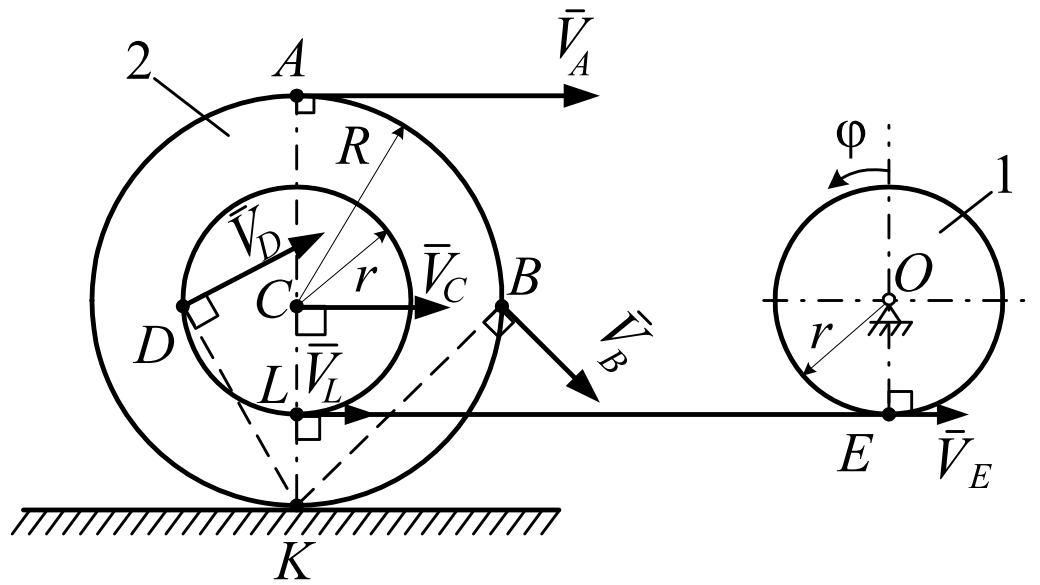
\includegraphics[width=0.99\textwidth]{lab3_task1_fig.png}\\
    \caption*{Task 1}
    \end{figure}
\end{minipage}
\end{frame}

\begin{frame}[c]{Task 2 (yours)
    }
\framesubtitle{}
    \vspace{-0.6cm}
    \begin{figure}[H]
        \centering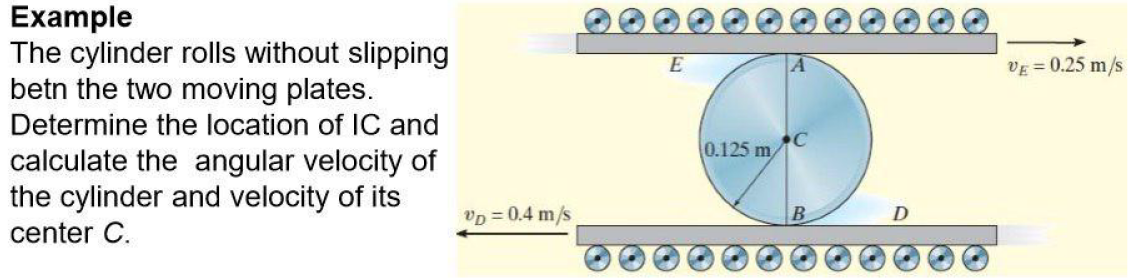
\includegraphics[height=6cm,width=1\textwidth,keepaspectratio]{image24.png}
        \label{fig:image24}
    \end{figure}
\end{frame}

\begin{frame}[t]{Task 2 (yours): tip}
\framesubtitle{}
    \vspace{-0.6cm}
    \begin{figure}[H]
        \centering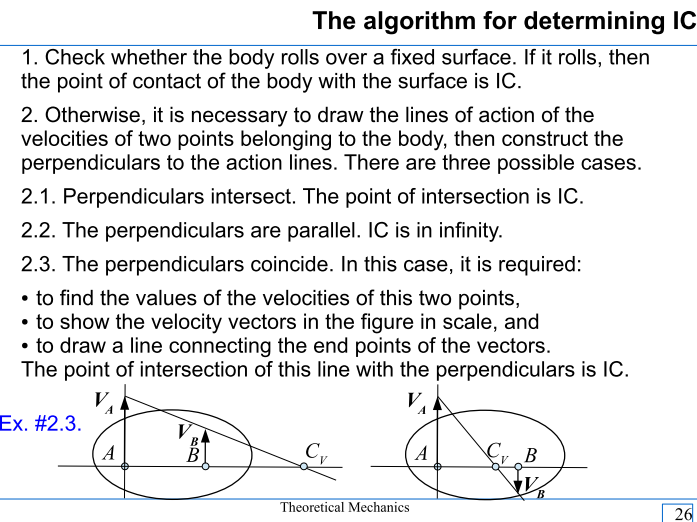
\includegraphics[height=6cm,width=1\textwidth,keepaspectratio]{image22.png}
        \label{fig:image22}
    \end{figure}
\end{frame}

\begin{frame}[t]{Task 2 (yours): solution}
\framesubtitle{}
    \vspace{-0.6cm}
    \begin{figure}[H]
        \centering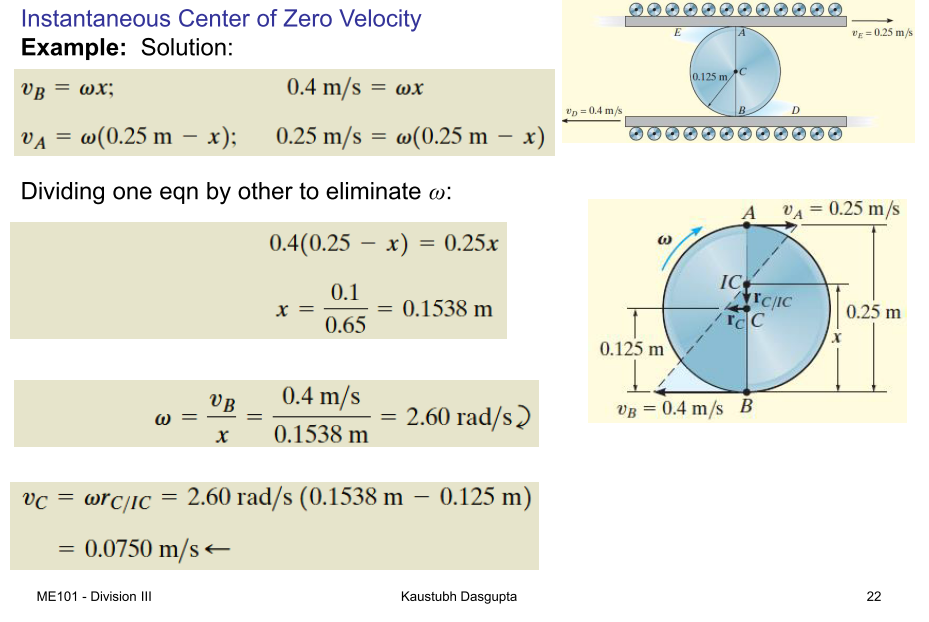
\includegraphics[height=6cm,width=1\textwidth,keepaspectratio]{image25.png}
        \label{fig:image25}
    \end{figure}
\end{frame}

\begin{frame}[t]{Task 3 (mine)}
    \framesubtitle{}
\begin{minipage}{0.6\textwidth}
The goal is to find velocities and accelerations (both direction and magnitude) of $A,\ B,\ C$ if you know all dimensions of the mechanism, $\omega_{OA}=2,\ \omega_1=1.2,\ \varepsilon_{OA}=0$.
\end{minipage}
\begin{minipage}{0.35\textwidth}
      \begin{figure}[H]
    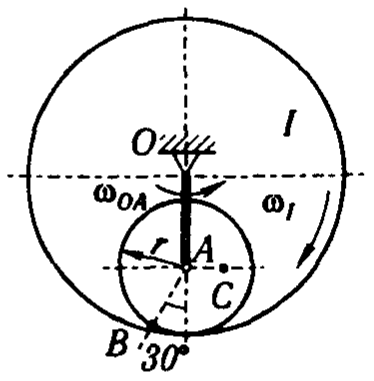
\includegraphics[width=0.99\textwidth]{lab3_task3_fig.png}\\
    \caption*{Task 3}
    \end{figure}
\end{minipage}
\end{frame}

\fbckg{fibeamer/figs/last_page.png}
\frame[plain]{}
\end{document}